
\subsection{定义}

拓扑排序的英文名是 Topological sorting。

拓扑排序要解决的问题是给一个图的所有节点排序。

我们可以拿大学选课的例子来描述这个过程, 比如学习大学课程中有: 单变量微积分, 线性代数, 离散数学概述, 概率论与统计学概述, 语言基础, 算法导论, 机器学习。 当我们想要学习 算法导论 的时候, 就必须先学会 离散数学概述 和 概率论与统计学概述, 不然在课堂就会听的一脸懵逼。 当然还有一个更加前的课程 单变量微积分。 这些课程就相当于几个顶点 $u$, 顶点之间的有向边 $(u,v)$ 就相当于学习课程的顺序。显然拓扑排序不是那么的麻烦, 不然你是如何选出合适的学习顺序。下面将介绍如何将这个过程抽象出来, 用算法来实现。

但是如果某一天排课的老师打瞌睡了, 说想要学习 算法导论, 还得先学 机器学习, 而 机器学习 的前置课程又是 算法导论, 然后你就一万脸懵逼了, 我到底应该先学哪一个 ? 当然我们在这里不考虑什么同时学几个课程的情况。在这里, 算法导论 和 机器学习 间就出现了一个环, 显然你现在没办法弄清楚你需要学什么了, 于是你也没办法进行拓扑排序了。因而如果有向图中存在环路, 那么我们就没办法进行 拓扑排序 了。

因此我们可以说 在一个 \href{/graph/dag}{DAG (有向无环图)} 中, 我们间图中的顶点以线性方式进行排序, 使得对于任何的顶点 $u$ 到 $v$ 的有向边  $(u,v)$  , 都可以有 $u$ 在 $v$ 的前面。

还有给定一个 \href{/graph/dag}{DAG (有向无环图)},如果从 $i$ 到 $j$ 有边,则认为 $j$ 依赖于 $i$。如果 $i$ 到 $j$ 有路径($i$ 可达 $j$),则称 $j$ 间接依赖于 $i$。

拓扑排序的目标是将所有节点排序,使得排在前面的节点不能依赖于排在后面的节点。

\subsection{Kahn 算法}

将入度为 0 的边组成一个集合 $S$ 

每次从 $S$ 里面取出一个顶点 $v$ (可以随便取) 放入  $L$, 然后遍历顶点 $v$ 的所有边$(u_1, v), (u_2, v), (u_3, v) \cdots$, 并删除, 并判断如果该边的另一个顶点, 如果在移除这一条边后入度为 0 , 那么就将这个顶点放入集合 $L$ 中。不断地重复取出顶点然后……

最后当集合为空后, 就检查图中是否存在任何边。如果有, 那么这个图一定有环路, 否者返回 $L$ , $L$ 中顺序就是拓扑排序的结果

首先看来自 \href{https://en.wikipedia.org/wiki/Topological_sorting#Kahn's_algorithm}{Wiki} 的伪代码

\vskip 0.2 in
\texttt{
L← Empty list that will contain the sorted elements\\S ← Set of all nodes with no incoming edges\\while S is non-empty do\\    remove a node n from S\\    insert n into L\\    for each node m with an edge e from n to m do\\        remove edge e from the graph\\        if m has no other incoming edges then\\            insert m into S\\if graph has edges then\\    return error (graph has at least onecycle)\\else \\    return L (a topologically sortedorder)}
\vskip 0.2 in

代码的核心是, 是维持一个入度为 0 的顶点。

可以参考该图

\begin{figure}[h]
\centering
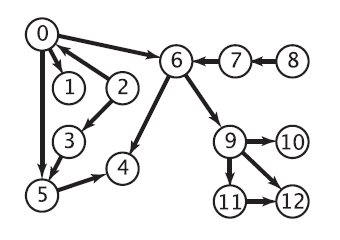
\includegraphics[width=0.5\textwidth]{images/1341373589_4609.png} 
\caption{1341373589_4609}
\end{figure}

对其排序的结果就是: 2 -> 8 -> 0 -> 3 -> 7 -> 1 -> 5 -> 6 -> 9 -> 4 -> 11 -> 10 -> 12

\subsubsection{时间复杂度}

假设这个图 $G = (V, E)$在初始化入度为 0 的集合 $S$ 的时候就需要遍历整个图, 并检查每一条边, 因而有 $\mathcal{O}(E+V)$ 的复杂度. 然后对该集合进行操作, 显然也是需要 $\mathcal{O}(E+V)$ 的时间复杂度。

因而总的时间复杂度就有 $\mathcal{O}(E+V)$

\subsubsection{实现}

伪代码:

\vskip 0.2 in
\texttt{
bool toposort() {\\	q = new queue();\\	for (i = 0; i < n; i++)\\		if (in_deg[i] == 0) q.push(i);\\	ans = new vector();\\	while (!q.empty()) {\\		u = q.pop();\\		ans.push_back(u);\\		for each edge(u, v) {\\			if (--in_deg[v] == 0) q.push(v);\\		}\\	}\\	if (ans.size() == n) {\\		for (i = 0; i < n; i++)\\			std::cout << ans[i] << std::endl;\\		return true;\\	} else {\\		return false;\\	}\\}}
\vskip 0.2 in

\subsection{DFS 算法}

\begin{cppcode}
// dfs 版本
bool dfs(int u) {
  c[u] = -1;
  for (int v = 0; v <= n; v++)
    if (G[u][v]) {
      if (c[v] < 0)
        return false;
      else if (!c[v])
        dfs(v);
    }
  c[u] = 1;
  topo.push_back(u);
  return true;
}
bool toposort() {
  topo.clear();
  memset(c, 0, sizeof(c));
  for (int u = 0; u <= n; u++)
    if (!c[u])
      if (!dfs(u)) return false;
  reverse(topo.begin(), topo.end());
  return true;
}
\end{cppcode}

时间复杂度:$O(n+m)$

空间复杂度:$O(n)$

\subsubsection{合理性证明}

考虑一个图,删掉某个入度为 0 的节点之后,如果新图可以拓扑排序,那么原图一定也可以。反过来,如果原图可以拓扑排序,那么删掉后也可以。

\subsection{参考}

\begin{enumerate}
\item 离散数学及其应用. ISBN:9787111555391
\item \href{https://blog.csdn.net/dm_vincent/article/details/7714519}{}
\item Topological sorting, \href{https://en.wikipedia.org/w/index.php?title=Topological_sorting&oldid=854351542}{}
\end{enumerate}
